\documentclass{article}

\usepackage{graphicx}
\usepackage{tikz}
\usepackage{tikzsymbols}
\usetikzlibrary{calc,patterns,shapes.geometric}
\pagestyle{empty}
\usepackage[margin=0pt]{geometry}
\geometry{papersize={14in,12in}}

\def\centerarc[#1](#2)(#3:#4:#5){\draw[#1] ($(#2)+({#5*cos(#3)},{#5*sin(#3)})$) arc (#3:#4:#5);}

\begin{document}
	\begin{figure}
		\centering
		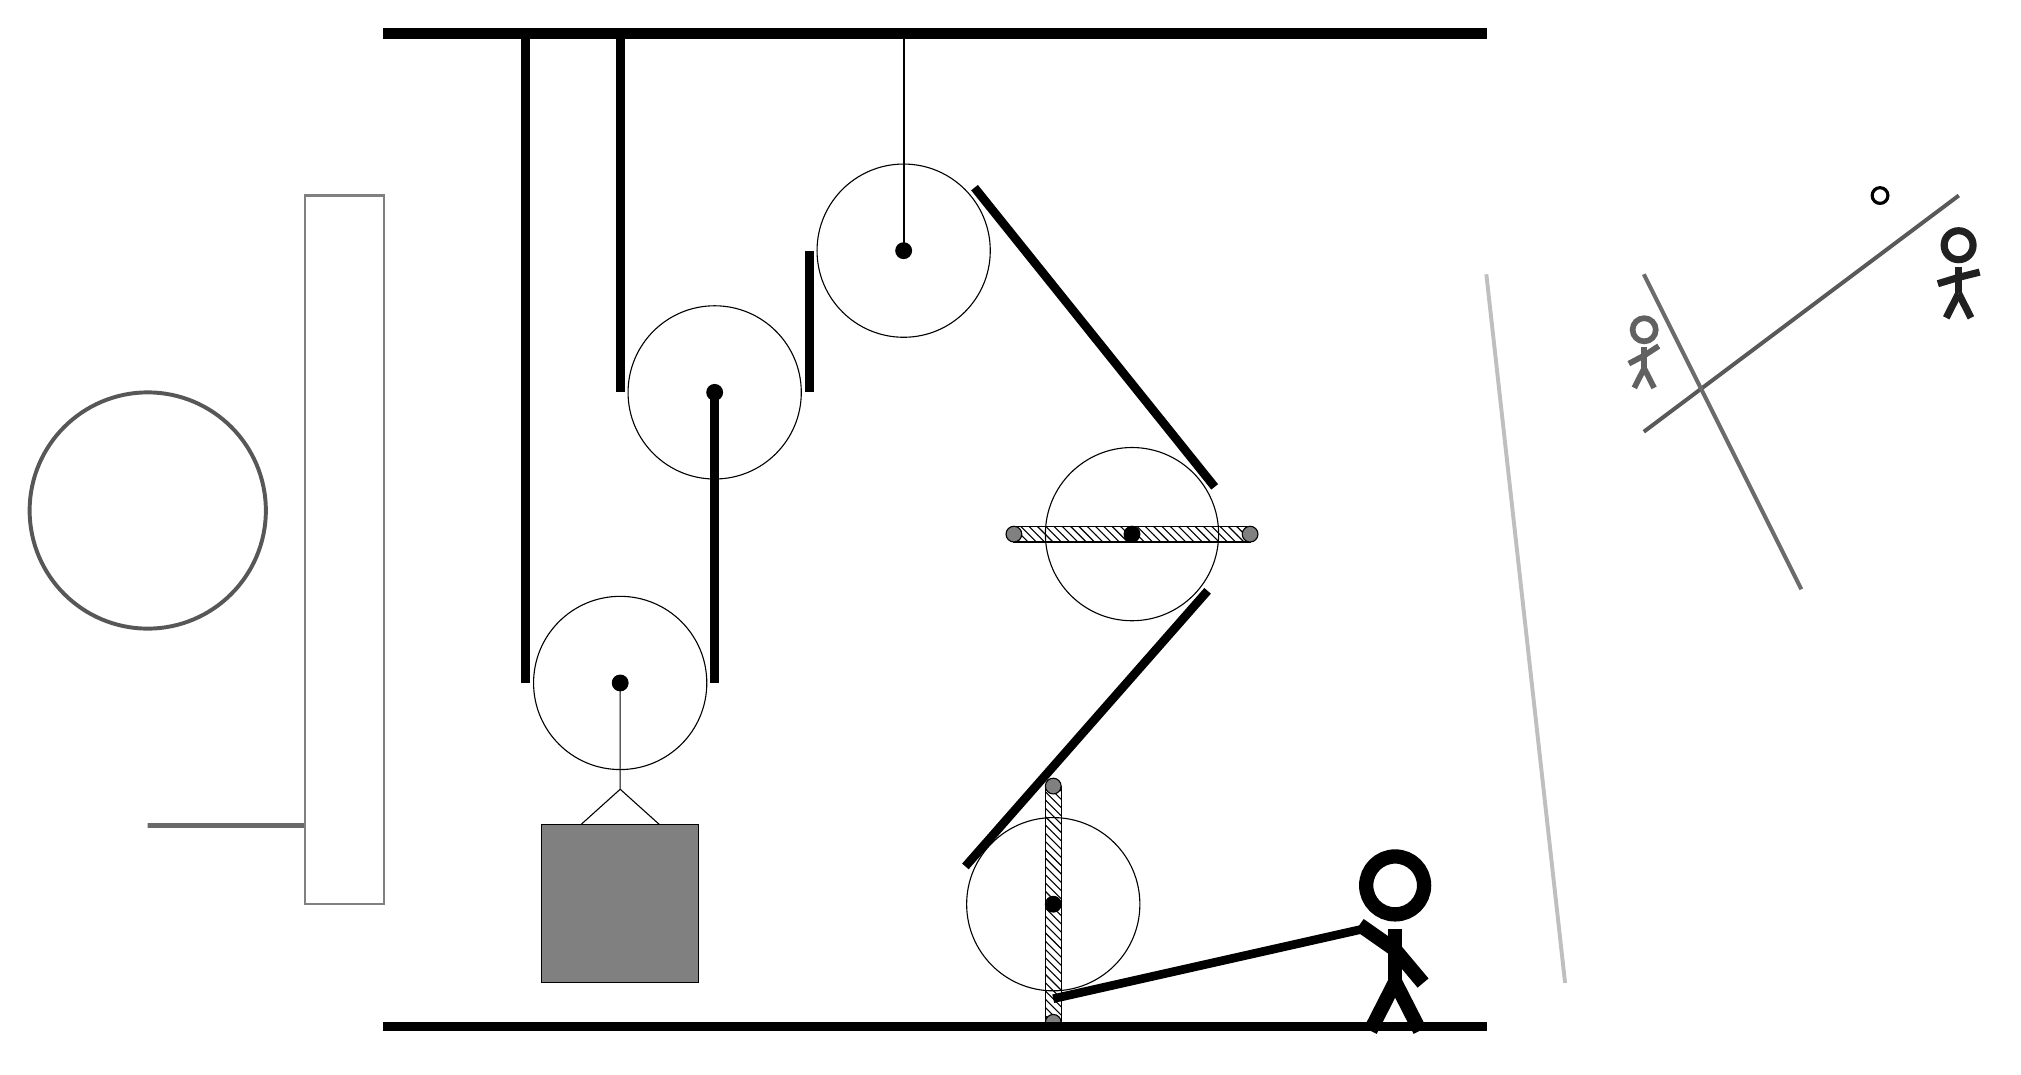
\begin{tikzpicture}
			%%%%% START %%%%%
			
			\draw[fill=black] (-2, 9) rectangle (12, 9.125);
			
			\draw[line width=0.5mm, color=black!65](14, 4) -- (18, 7);
			
			\node[line width=0.6mm, color=black!87] at (18, 6) {\Strichmaxerl[5][17][14]};
			\draw[line width=0.5mm, color=black!25](13, -3) -- (12, 6);
			\draw[line width=0.5mm, color=black!58](16, 2) -- (14, 6);
			\draw [line width=0.5mm, color=black!66](-5, 3) circle (1.5);
			\draw[line width=0.7mm, color=black!59] (-3, -1) rectangle (-5, -1);
			\node[line width=0.2mm, color=black!62] at (14, 5) {\Strichmaxerl[4][28][33]};
			\draw[line width=0.3mm, color=black!50] (-2, -2) rectangle (-3, 7);
			\draw [line width=0.4mm, color=black!100](17, 7) circle (0.1);
			
			\draw (1, 0.81) circle (1.1);
			\draw[fill=black] (1, 0.81) circle (0.1);
			
			\draw (2.2, 4.5) circle (1.1);
			\draw[fill=black] (2.2, 4.5) circle (0.1);
			
			\draw (4.6, 6.3) circle (1.1);
			\draw[fill=black] (4.6, 6.3) circle (0.1);
			\draw[thick] (4.6, 6.3) -- (4.6, 9);
			
			\draw (6.5, -2) circle (1.1);
			\draw[fill=black] (6.5, -2) circle (0.1);
			\draw[pattern=north west lines, pattern color=black] (6.4, -0.5) rectangle (6.6, -3.5);
			\draw[fill=black!50] (6.5, -0.5) circle (0.1);
			\draw[fill=black!50] (6.5, -3.5) circle (0.1);
			
			\draw (7.5, 2.7) circle (1.1);
			\draw[fill=black] (7.5, 2.7) circle (0.1);
			\draw[pattern=north west lines, pattern color=black] (6.0, 2.8) rectangle (9.0, 2.6);
			\draw[fill=black!50] (6.0, 2.7) circle (0.1);
			\draw[fill=black!50] (9.0, 2.7) circle (0.1);
			
			\draw (1, 0.81) -- (1, -0.54) -- (0.5, -0.99) -- (1.5, -0.99) -- (1, -0.54);
			\draw[fill=black!50] (0, -0.99) rectangle (2, -2.99);
			
			\draw[line width=1.1mm] (-0.2, 9) -- (-0.2, 0.81);
			\centerarc[line width=1.1mm](1, 0.81)(180:360:1.2000000000000002);
			\draw[line width=1.1mm](2.2, 0.81) -- (2.2, 4.5);
			\draw[line width=1.1mm] (1.0, 9) -- (1.0, 4.5);
			\centerarc[line width=1.1mm](2.2, 4.5)(180:360:1.2000000000000002);
			\draw[line width=1.1mm](3.4, 4.5) -- (3.4, 6.3);
			\centerarc[line width=1.1mm](4.6, 6.3)(35:180:1.2000000000000002);
			\draw[line width=1.1mm] (5.5, 7.1) -- (8.55, 3.3);
			\centerarc[line width=1.1mm](7.5, 2.7)(215:135:-1.2000000000000002);
			\draw[line width=1.1mm](8.46, 1.98) -- (5.384, -1.52);
			\centerarc[line width=1.1mm](6.5, -2)(-30:100:-1.2000000000000002);
			\draw[line width=1.1mm](6.5, -3.2) -- (10.5, -2.3);
			
			\node at (10.8, -2.5) {\Strichmaxerl[10][-35][-50]};
			
			\draw[fill=black] (-2, -3.5) rectangle (12, -3.6);
			
			%%%%% END %%%%%
		\end{tikzpicture}
	\end{figure}	
\end{document}